\ifdefined\pdfminorversion\pdfminorversion=6\fi
\documentclass[conference,a4paper]{IEEEtran}

\usepackage{amsmath}
\usepackage{graphicx}
\usepackage{booktabs}
\usepackage{cite}
\usepackage[hidelinks]{hyperref}

% Target venue constraint: IEEE conference format, A4 paper, up to 6 pages.

\title{Nine-Dash Line Detection: A Moderation-Oriented Benchmark with Hard-Negative Region Distillation}

\author{
\IEEEauthorblockN{First Author\IEEEauthorrefmark{1}, Second Author\IEEEauthorrefmark{2}, and Third Author\IEEEauthorrefmark{1}}
\IEEEauthorblockA{\IEEEauthorrefmark{1}Department or Laboratory, University or Organization\\
Email: first.author@example.edu, third.author@example.edu}
\IEEEauthorblockA{\IEEEauthorrefmark{2}Department or Laboratory, University or Organization\\
Email: second.author@example.edu}
}

\begin{document}
\maketitle

\begin{abstract}
Detecting the nine-dash line in real-world imagery is difficult because the target is often small, fragmented, and similar to ordinary map strokes. We introduce a public benchmark of 7,344 images and 2,636 annotated objects, including positive images, in-domain map-like negatives, and out-of-domain negatives. Faster R-CNN, SSD, and YOLO-family detectors are evaluated with object-level and moderation-oriented metrics. We also propose HN-SARD, a Hard-Negative and Scale-Aware Region Distillation framework that uses a frozen DINOv2 teacher to regularize Faster R-CNN region features. Explicit negative training substantially reduces false positives, while HN-SARD improves AP and selected moderation metrics over its base detector.
\end{abstract}

\begin{IEEEkeywords}
nine-dash line detection, object detection, visual moderation, hard negatives, knowledge distillation, DINOv2
\end{IEEEkeywords}

\section{Introduction}
The nine-dash line may appear in maps, screenshots, posters, and printed materials. Unlike a compact logo, it consists of thin, disconnected strokes whose appearance varies with map style, resolution, compression, color palette, and surrounding geography. The same visual vocabulary occurs in coastlines, borders, routes, bathymetric marks, and grid lines. A detector must therefore recover small or low-contrast targets without over-triggering on ordinary map content.

Object-level AP alone does not characterize a moderation system: operational use also requires high image recall with few false alarms. A model with good localization can still create an excessive review queue if it fires on clean maps. Conversely, a conservative threshold may suppress false positives by missing positive images. We consequently treat screening as a joint localization and image-decision task and evaluate both bounding-box quality and false-positive behavior on realistic map-like and unrelated negatives.

This paper makes three contributions:
\begin{itemize}
    \item We release a public real-world benchmark with positive images and both in-domain and out-of-domain negatives.
    \item We define a moderation-oriented evaluation protocol that combines COCO-style detection metrics with image-level false-positive metrics.
    \item We propose and ablate HN-SARD (Hard-Negative and Scale-Aware Region Distillation), a DINOv2-based module for improving false-positive-oriented behavior of a Faster R-CNN detector.
\end{itemize}

\section{Related Work}
\textbf{Object detection.}
Faster R-CNN \cite{ren2015faster} separates region proposal and RoI classification, while FPN supports multi-scale features \cite{lin2017fpn}. Its explicit candidates are useful here because they expose foreground-like regions before the final decision. SSD \cite{liu2016ssd} and YOLO \cite{redmon2016you} instead provide one-stage speed--accuracy tradeoffs, and recent YOLO variants are competitive deployment baselines \cite{wang2024yolov9,wang2024yolov10,ultralytics2024yolo11}. We compare proposal-based, classical one-stage, and recent YOLO detectors under one data and evaluation protocol.

\textbf{Tiny and thin object detection.}
Sparse line segments are sensitive to downsampling and multi-scale representation \cite{lin2017fpn,kisantal2019augmentation}. A box enclosing several dashes may become only a few pixels wide after resizing while remaining surrounded by complex map strokes. Absolute COCO area thresholds do not capture this dependence on source resolution, so we use relative-area groups: tiny $<1\%$, small $1$--$5\%$, medium $5$--$25\%$, and large $\geq25\%$. This stratification reveals scale sensitivity without treating the limited tiny subset as a standalone benchmark.

\textbf{Hard negatives and false-positive control.}
Hard-negative methods include online mining \cite{shrivastava2016ohem}, loss re-weighting \cite{lin2017focal}, and classification refinement \cite{cheng2018dcr}. These approaches emphasize difficult background rather than uniformly sampling easy negatives. Because high AP can coexist with many false alarms, we make in-domain and out-of-domain negatives explicit training and evaluation groups and report both threshold-dependent image errors and the number of false boxes.

HN-SARD differs from selecting examples solely by detector loss. It first restricts attention to foreground-like proposals that have little overlap with any target, then regularizes their region representation against a queue of positive teacher anchors. Thus, the auxiliary signal acts on the feature geometry of current false-positive candidates, while the standard detector loss continues to supervise classification and localization.

\textbf{Distillation from foundation models.}
HN-SARD follows teacher--student distillation \cite{hinton2015distilling} but uses a frozen self-supervised teacher on region crops and emphasizes hard negatives \cite{li2022rank}. DINO and DINOv2 provide strong general-purpose visual representations \cite{caron2021dino,oquab2023dinov2}. Our region-level design differs from full-image distillation: resizing a matched context crop to the teacher input gives small symbolic details more pixels while retaining nearby map evidence. The teacher supplies only an auxiliary training signal and does not replace detection supervision.

The positive and negative terms also use the teacher asymmetrically. Positive RoIs are aligned with their corresponding DINOv2 crop embeddings, whereas negative RoIs are not assigned artificial teacher targets. Instead, their student embeddings are separated from recent positive anchors. This avoids treating diverse background regions as a single semantic class in the teacher space.

\section{Dataset}
\subsection{Data Organization}
Public Internet images were organized as \texttt{positive}, \texttt{negative\_in\_domain}, or \texttt{negative\_out\_domain}. Positives contain annotated nine-dash-line boxes; in-domain negatives are target-free maps or geographic diagrams; and out-of-domain negatives are unrelated images. The two negative groups serve different purposes: one stresses visually plausible map confusion, while the other measures broad-domain robustness. Their separation prevents map-specific errors from being hidden among easy negatives.

Each record contains the file name, image size, split, and clipped $(x,y,w,h)$ boxes; negatives use an empty object list. The released package provides the images, human annotations, split metadata, attribution, and common evaluation code. Images are cleared for academic redistribution, with source attribution where required. This uniform representation supports object metrics, image-level decisions, and group-specific false-positive analysis without separate loaders.

Table~\ref{tab:dataset} summarizes the resulting split sizes and object counts.

\begin{table}[!h]
\centering
\caption{Dataset statistics by split.}
\label{tab:dataset}
\resizebox{\linewidth}{!}{
\begin{tabular}{lrrrrrr}
\toprule
Split & Pos. img. & Neg.-ID & Neg.-OOD & Neg. total & Images & Objects \\
\midrule
Train & 1,642 & 2,048 & 1,451 & 3,499 & 5,141 & 1,837 \\
Val   &   352 &   439 &   311 &   750 & 1,102 &   402 \\
Test  &   351 &   439 &   311 &   750 & 1,101 &   397 \\
\midrule
Total & 2,345 & 2,926 & 2,073 & 4,999 & 7,344 & 2,636 \\
\bottomrule
\end{tabular}}
\end{table}

\subsection{Annotation and Split Protocol}
Annotators placed one box around each visible nine-dash-line cluster rather than individual dashes. This cluster-level convention matches moderation: a detection should direct a reviewer to the symbol region rather than segment every stroke. A second pass checked target presence, box coverage, coordinates, and negative labels; ambiguous images were handled conservatively.

Every split contains the same semantic groups. Validation and test each contain 439 in-domain and 311 out-of-domain negatives, making validation operating-point selection comparable to test reporting. Duplicate, near-duplicate, and source-related images were kept within one split to limit leakage. Images are loaded deterministically by group and file name; all models use the fixed \texttt{canonical\_v2} split and seed 42 rather than regenerating partitions per experiment.

Fixing the negative composition is particularly important because FPR can change even when object AP is nearly unchanged. A regenerated split could alter the proportion of easy photographs and hard maps, obscuring whether an improvement comes from training or test composition. The shared split therefore supports controlled comparison across detector families and ablations.

The test set has only 15 tiny instances. Many visible targets are medium or large relative to their source image, whereas truly tiny examples are difficult to collect and annotate consistently. Tiny AP is therefore treated as a diagnostic of scale sensitivity rather than a claim of general tiny-object state of the art.

Fig.~\ref{fig:dataset_examples} illustrates the positive, in-domain negative, and out-of-domain negative image groups used by the benchmark.

\begin{figure}[!h]
\centering
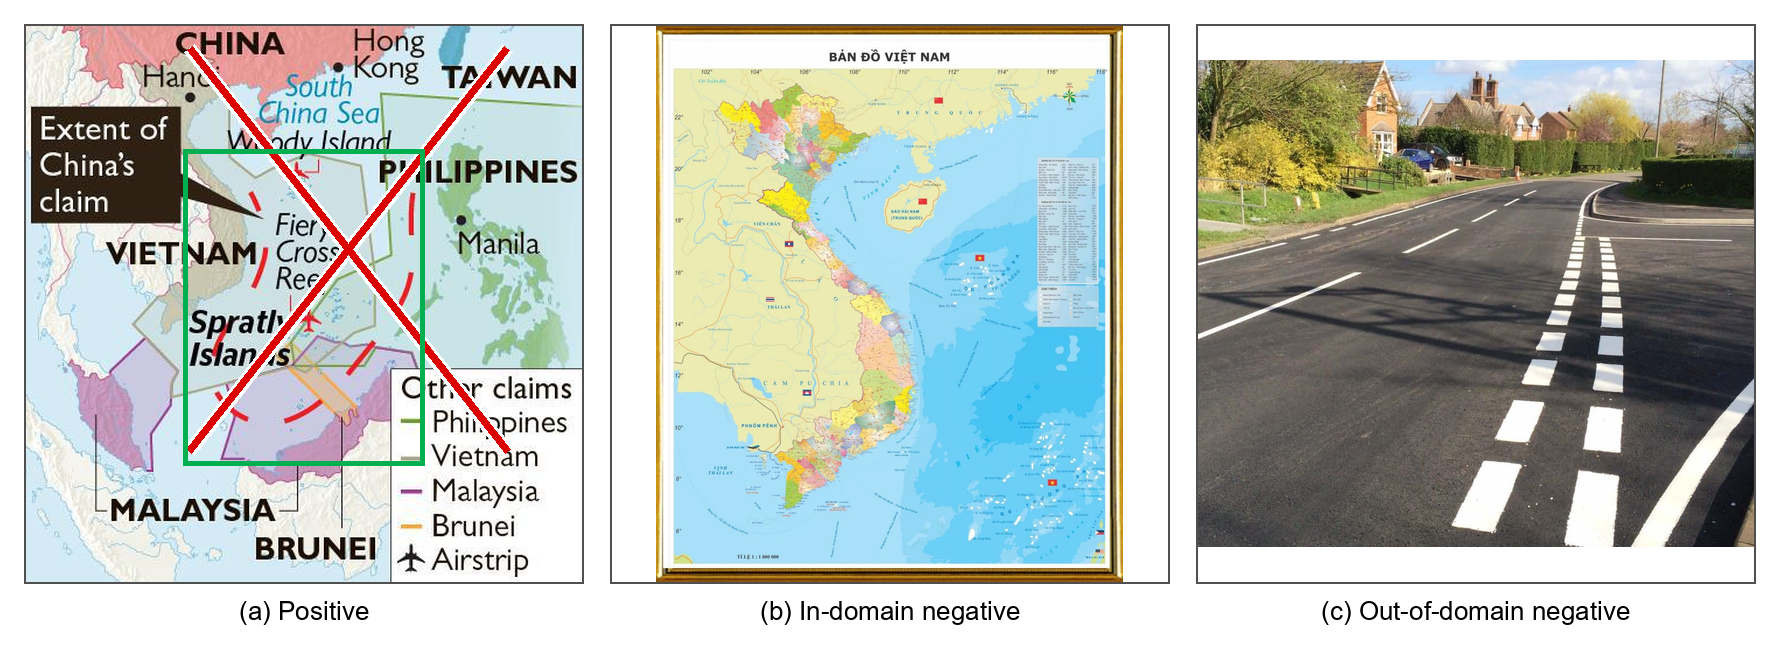
\includegraphics[width=\columnwidth]{fig1_dataset_examples.png}
\caption{Dataset examples: (a) positive, (b) in-domain negative, and (c) out-of-domain negative. The red X marks the target region.}
\label{fig:dataset_examples}
\end{figure}

\begin{figure*}[!t]
    \centering
    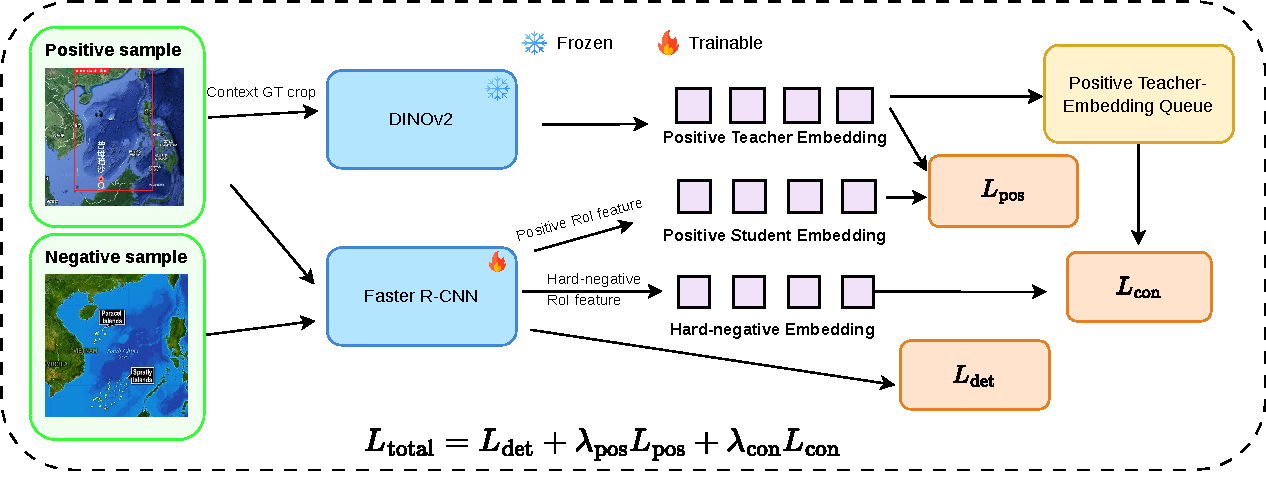
\includegraphics[width=0.9\textwidth]{architecture.pdf}
    \caption{HN-SARD training overview. The DINOv2 teacher is frozen and only receives context crops; the Faster R-CNN student receives full images.}
    \label{fig:hnsard_pipeline}
\end{figure*}

\subsection{Evaluation Metrics}
Object-level metrics follow COCO bounding-box evaluation \cite{lin2014coco}: AP, AP50, AP75, and AR@100 (AR in tables), with AP also computed by relative-area group. Given detection confidences $\{c_j\}_{j=1}^{m}$, the image-level moderation score is
\begin{equation}
s(I)=
\begin{cases}
\max_j c_j, & m>0,\\
0, & m=0.
\end{cases}
\end{equation}
Thus, one high-confidence box is sufficient to flag an image. We report AUROC, FPR@95TPR, recall at FPR budgets of 1\% and 5\% (R@1\%FPR and R@5\%FPR), and group-specific FPR.

At threshold $t$, let TP, FP, TN, and FN denote image-level counts. The false-positive rate is
\begin{equation}
\mathrm{FPR}(t)=\frac{\mathrm{FP}(t)}{\mathrm{FP}(t)+\mathrm{TN}(t)}.
\end{equation}
FPR@95TPR is the minimum FPR among thresholds reaching at least 95\% TPR; FPR-ID and FPR-OOD are its in- and out-of-domain components. R@1\%FPR and R@5\%FPR are the highest attainable recalls under the stated false-positive budgets. Reporting both directions exposes models that obtain low FPR only by missing positives.

Negative FPPI is measured at the diagnostic threshold $t=0.25$:
\begin{equation}
\mathrm{FPPI}=\frac{\#\{\text{detections on negative images}\}}
{\#\{\text{negative images}\}}.
\end{equation}
Unlike FPR, FPPI counts multiple boxes per image and therefore estimates the box-level noise presented to a reviewer. The fixed threshold supports comparable diagnostics; deployment thresholds should instead be selected on validation data for the desired review budget.

These metrics provide complementary views. AUROC summarizes ranking over all thresholds but may hide behavior in the low-FPR region. FPR@95TPR fixes a high-recall requirement, while R@1\%FPR and R@5\%FPR reverse the constraint and expose attainable recall under limited review budgets. Group-specific FPR then identifies whether the remaining errors arise from map-like or unrelated content.

\section{Method}
\subsection{Overview}
HN-SARD addresses two complementary failure modes: weak positive evidence for small or thin targets and foreground-like responses on negative maps. Scale-aware positive distillation aligns student RoI features with frozen DINOv2 embeddings of ground-truth context crops. In parallel, contrastive distillation separates high-scoring low-IoU proposals from recent positive teacher embeddings. During training, positive RoIs are aligned with frozen DINOv2 crop embeddings, while high-scoring low-IoU proposals are separated from queued positive anchors. At inference, the teacher, crop encoder, hard-negative mining, and anchor queue are removed, leaving the standard Faster R-CNN prediction path unchanged.

Fig.~\ref{fig:hnsard_pipeline} summarizes the HN-SARD training flow and the separation between frozen teacher crops and full-image student detection.

\subsection{Base Detector}
HN-SARD uses Faster R-CNN R50-FPN because its proposals and explicit RoI features provide direct teacher--student region correspondences and a natural pool for hard-negative mining \cite{ren2015faster}. By contrast, a dense YOLO host would require a new mechanism to form regions, establish teacher--student correspondences, and mine proposal-like negatives. Such changes would confound evaluation of the auxiliary losses, so YOLO models remain strong benchmark baselines rather than direct HN-SARD hosts.

The standard detector loss is
\begin{equation}
L_{\mathrm{det}} = L_{\mathrm{rpn-cls}} + L_{\mathrm{rpn-reg}} + L_{\mathrm{roi-cls}} + L_{\mathrm{roi-reg}}.
\end{equation}
A linear projection after the RoI box head maps student features to the teacher dimension. The prediction head is unchanged, and the teacher is absent at inference.

\subsection{Frozen DINOv2 Teacher}
For a matched ground-truth box $(x,y,w,h)$ with center $(c_x,c_y)$, context scale $k$ gives dimensions
\begin{equation}
w'=kw, \qquad h'=kh.
\end{equation}
The crop bounds are
\begin{equation}
\begin{aligned}
x'_1&=\max(0,c_x-w'/2), & y'_1&=\max(0,c_y-h'/2),\\
x'_2&=\min(W,c_x+w'/2), & y'_2&=\min(H,c_y+h'/2),
\end{aligned}
\end{equation}
for image dimensions $(W,H)$. The default $k=1.5$ enlarges both box dimensions by 50\% while keeping the center fixed. The added context includes nearby strokes and labels that may distinguish the symbol from an isolated dash. Crops are taken from the original image before detector resizing, resized to $224\times224$, normalized with the teacher processor statistics, and encoded by frozen \texttt{facebook/dinov2-small}. Its 384-dimensional final-layer CLS token is the teacher embedding.

\subsection{Positive Region Distillation}
Let $\hat{z}^{S}_{i}$ be the normalized projected student embedding for proposal $i$, and let $\hat{z}^{T}_{i}$ be the normalized teacher embedding for its matched context crop. In the selected scale-aware setting, the positive distillation term is a weighted cosine distance,
\begin{equation}
L_{\mathrm{pos}} =
\frac{\sum_{i \in P} w_i \left(1 - \hat{z}^{S}_{i} \cdot \hat{z}^{T}_{i}\right)}
{\sum_{i \in P} w_i}.
\end{equation}
The area weight $w_i$ is 1.5 for boxes below 1\% of image area, 1.25 for 1--5\%, and 1 otherwise, preventing large or easy objects from dominating the auxiliary signal. Eligible proposals have IoU $\geq0.5$; up to 16 per image are sampled by first retaining the highest-IoU proposal for each object and then filling the budget with other high-IoU proposals.

\subsection{Online Hard-Negative Contrastive Distillation}
From the top 128 RPN proposals, candidates are those with maximum ground-truth IoU below 0.1, or all proposals in a negative image. Proposals with $0.1\leq\mathrm{IoU}<0.5$ receive neither auxiliary loss but retain the detector loss. The 16 candidates with highest foreground scores become hard negatives. For normalized negative embedding $\hat{z}^{N}_{j}$ and positive-teacher queue $\mathcal{B}$, define
\begin{equation}
s_j = \max_{a \in \mathcal{B}} \hat{z}^{N}_{j} \cdot a .
\end{equation}
The softplus contrastive loss over hard-negative set $\mathcal{N}$ is
\begin{equation}
L_{\mathrm{con}} =
\frac{1}{|\mathcal{N}|}\sum_{j \in \mathcal{N}}
\tau \log\left(1 + \exp\left(\frac{s_j - m}{\tau}\right)\right),
\end{equation}
with margin $m=0.2$, temperature $\tau=0.1$, and queue size 512. The soft margin increasingly penalizes negatives similar to any positive anchor without imposing a hard cutoff; negatives below the margin retain a small nonzero penalty. The full objective is
\begin{equation}
L = L_{\mathrm{det}} + \lambda_{\mathrm{pos}}L_{\mathrm{pos}} + \lambda_{\mathrm{con}}L_{\mathrm{con}},
\end{equation}
Validation selects $\lambda_{\mathrm{pos}}=0.0025$ and $\lambda_{\mathrm{con}}=0.02$. The contrastive weight is zero for epochs 1--5 and 0.02 thereafter. Hard-negative mining is online because it uses the current detector scores rather than a static negative list: as training changes, different proposals enter the top-16 set. Detached positive teacher embeddings are enqueued before evaluating the batch contrastive term, so current positives can act as anchors immediately. The FIFO queue retains only the 512 most recent anchors and carries information across batches; when none is available, $L_{\mathrm{con}}=0$. Ablations disable either or both auxiliary terms.

\section{Experiments}
\subsection{Protocol}
Models train for at most 50 epochs with batch size 8, validation each epoch, and early-stopping patience 15. Torchvision models use 800--1333-pixel resizing; YOLO uses 960 pixels. Augmentation comprises horizontal flipping ($p=0.5$) and brightness, saturation, and hue jitter of 0.2, 0.2, and 0.015. YOLO-specific mosaic, mixup, copy-paste, geometric, and perspective transforms are disabled to keep the comparison conservative.

Faster R-CNN uses SGD (learning rate 0.005, momentum 0.9, weight decay 0.0005) and StepLR every five epochs; SSD uses learning rate 0.002 and gradient clipping. Ultralytics YOLO outputs are re-evaluated by the common metric code. Validation controls checkpoints, early stopping, and every HN-SARD hyperparameter using both detection and false-positive behavior. Configurations are frozen before test evaluation; consequently, the reported loss grid is a held-out sensitivity analysis rather than test-based selection.

The main detector comparison, dataset ablation, loss-weight ablation, and error audit use the held-out test split. The context-scale study is explicitly a validation diagnostic because crop scale is a training hyperparameter. All result directories record the split protocol and seed, and all detector outputs pass through the same post-training evaluator. This separation prevents test metrics from determining the selected HN-SARD configuration.

\subsection{Baseline Comparison}
Table~\ref{tab:baselines} compares held-out test performance; it is not a speed benchmark or exhaustive leaderboard.

\begin{table*}[!t]
\centering
\caption{Test-set comparison of detectors.}
\label{tab:baselines}
\resizebox{\linewidth}{!}{
\begin{tabular}{lrrrrrrrrr}
\toprule
Method & AP & AP50 & AP$_t$ & AR & Img. AUROC & R@1\%FPR & R@5\%FPR & FPR@95 & Neg. FPPI \\
\midrule
Faster R-CNN R50-FPN & 0.685 & \textbf{0.966} & 0.325 & 0.747 & 0.986 & 0.940 & 0.974 & 0.012 & 0.096 \\
Faster R-CNN R101-FPN & 0.617 & 0.939 & 0.255 & 0.691 & 0.993 & 0.886 & 0.974 & 0.032 & 0.120 \\
SSD300 VGG16 & 0.673 & 0.888 & 0.206 & 0.768 & 0.962 & 0.575 & 0.832 & 0.151 & 0.317 \\
YOLOv8s & 0.731 & 0.954 & 0.343 & 0.775 & 0.986 & 0.946 & 0.972 & 0.011 & 0.005 \\
YOLOv9s & \textbf{0.747} & 0.953 & 0.336 & \textbf{0.791} & 0.987 & 0.957 & 0.977 & \textbf{0.003} & \textbf{0.003} \\
YOLOv10s & 0.735 & 0.935 & 0.321 & 0.782 & 0.985 & 0.957 & 0.972 & 0.005 & \textbf{0.003} \\
YOLO11s & 0.743 & 0.955 & 0.331 & 0.785 & 0.984 & 0.929 & 0.972 & 0.016 & 0.007 \\
Faster R-CNN + HN-SARD (Ours) & 0.713 & \textbf{0.966} & \textbf{0.367} & 0.766 & \textbf{0.996} & \textbf{0.960} & \textbf{0.980} & 0.007 & 0.055 \\
\bottomrule
\end{tabular}}
\end{table*}

YOLOv9s has the highest AP and AR, while YOLOv9s and YOLOv10s also produce the lowest negative FPPI. HN-SARD does not surpass the strongest YOLO models in overall AP, but it improves AP, tiny AP, FPR@95TPR, and both fixed-budget recalls over its Faster R-CNN base while matching AP50. Its image AUROC of 0.996 is also the highest in the comparison. SSD's reasonable AP but weak low-FPR recall illustrates why localization and moderation metrics are complementary: models with similar AP can create substantially different review loads. Faster R-CNN remains useful for proposal-level analysis even though the strongest YOLO models achieve better overall detection results. Tiny AP remains the weakest regime and should be interpreted cautiously given the small number of tiny test objects.

The ranking also depends on the operational objective. YOLOv9s is the strongest general detector in this set, whereas HN-SARD provides the clearest controlled gain over a proposal-based parent. Its lower FPPI and higher fixed-budget recall relative to Faster R-CNN show that auxiliary supervision changes more than bounding-box localization. We therefore treat the YOLO rows as competitive benchmark context and the Faster R-CNN pair as the direct test of HN-SARD.

\subsection{Dataset Ablation}
Table~\ref{tab:dataset_ablation} measures the effect of negative training data.

\begin{table}[!t]
\centering
\caption{Faster R-CNN dataset ablation.}
\label{tab:dataset_ablation}
\resizebox{\linewidth}{!}{
\begin{tabular}{lrrrrrr}
\toprule
Training data & AP & AP50 & FPR-ID & FPR-OOD & FPR@95 & Neg. FPPI \\
\midrule
Positive only & 0.672 & 0.943 & 0.103 & 0.068 & 0.088 & 0.889 \\
Pos. + neg.-OOD & 0.674 & 0.951 & 0.096 & \textbf{0.000} & 0.056 & 0.348 \\
Pos. + neg.-ID & 0.682 & \textbf{0.966} & 0.027 & 0.013 & 0.021 & 0.191 \\
Pos. + Neg.-ID + Neg.-OOD & \textbf{0.685} & \textbf{0.966} & \textbf{0.021} & \textbf{0.000} & \textbf{0.012} & \textbf{0.096} \\
\bottomrule
\end{tabular}}
\end{table}

Negatives have little effect on AP but sharply improve moderation behavior. In-domain negatives are more valuable for map-like confusion, reducing FPR-ID from 0.103 to 0.027, whereas out-of-domain negatives eliminate most unrelated-image errors but leave substantial in-domain FPR. This asymmetry confirms that unrelated photographs are not an adequate substitute for visually plausible clean maps. Using both groups gives the best balance, lowering FPR@95TPR from 0.088 to 0.012 and FPPI from 0.889 to 0.096 while slightly increasing AP. The result also explains why an object-only evaluation would understate the contribution of negative training data.

The four rows further separate coverage from specialization. Out-of-domain negatives reduce broad visual over-triggering, but a model trained without clean maps still confuses target-like cartographic strokes. In-domain negatives address this harder boundary and also generalize reasonably to unrelated images. Combining the groups covers both failure sources and yields the only configuration that minimizes every reported false-positive measure simultaneously.

\subsection{HN-SARD Loss-Weight Ablation}
Table~\ref{tab:loss_ablation} separates the positive and contrastive terms and tests the validation-selected weights on the held-out test set.

\begin{table}[!t]
\centering
\caption{HN-SARD loss-weight ablation.}
\label{tab:loss_ablation}
\resizebox{\linewidth}{!}{
\begin{tabular}{lrrrrrrr}
\toprule
Variant & $\lambda_{\mathrm{pos}}$ & $\lambda_{\mathrm{con}}$ & AP & AP$_t$ & FPR-ID & R@1\%FPR & Neg. FPPI \\
\midrule
Baseline & 0 & 0 & 0.685 & 0.325 & 0.021 & 0.940 & 0.096 \\
Contrastive only & 0 & 0.02 & 0.707 & \textbf{0.388} & 0.016 & 0.954 & 0.065 \\
Positive only & 0.0025 & 0 & 0.708 & 0.371 & \textbf{0.011} & \textbf{0.960} & 0.075 \\
Selected HN-SARD & 0.0025 & 0.02 & \textbf{0.713} & 0.367 & \textbf{0.011} & \textbf{0.960} & \textbf{0.055} \\
Positive only (higher weight) & 0.005 & 0 & 0.712 & 0.333 & 0.016 & 0.952 & 0.068 \\
Large weight & 0.05 & 0.05 & 0.692 & 0.329 & 0.027 & 0.940 & 0.061 \\
\bottomrule
\end{tabular}}
\end{table}

The selected HN-SARD setting raises AP from 0.685 to 0.713, tiny AP from 0.325 to 0.367, and R@1\%FPR from 0.940 to 0.960 while reducing FPPI from 0.096 to 0.055. These simultaneous changes indicate that false-positive reduction does not come merely from suppressing all detections. Contrastive-only gives the highest tiny AP but higher FPPI, suggesting that separation from positive anchors helps scale-sensitive representation but does not fully control the number of emitted boxes. Positive-only matches the selected setting's rounded FPR-ID and recall but also has higher FPPI. The higher-positive-weight setting nearly matches selected AP but disables hard-negative contrast and increases FPPI. Large weights degrade AP and FPR-ID, supporting DINOv2 supervision as a small regularizer rather than a replacement for detection loss.

Because the combined weights were chosen on validation, the test grid should be read as sensitivity analysis rather than a second model-selection stage. The close AP values among the small-weight variants indicate a stable region, while their FPPI differences reveal behavior that AP alone cannot resolve. The selected setting is therefore retained for its joint localization and review-noise balance, not because every individual column is optimal.

\subsection{Ground-Truth Context-Scale Ablation}
Table~\ref{tab:gt_scale_ablation} evaluates teacher-crop scale $k$ on validation with fixed $\lambda_{\mathrm{pos}}=0.0025$ and $\lambda_{\mathrm{con}}=0.02$. AP$_t$ and AP$_s$ cover objects below 1\% and within 1--5\% of image area. The default $k=1.5$ gives the highest overall AP, lowest FPR-ID, and best fixed-budget recall. However, $k=1.0$ favors tiny AP and $k=2.0$ favors small AP, so no scale leads every metric. This sensitivity supports moderate context rather than assuming that more surrounding map content is always beneficial.

\begin{table}[t]
\centering
\caption{Teacher-crop context-scale ablation.}
\label{tab:gt_scale_ablation}
\scriptsize
\setlength{\tabcolsep}{1.4pt}
\begin{tabular}{@{}crrrrrrr@{}}
\toprule
$k$ & AP & AP$_t$ & AP$_s$ & FPR-ID & FPR@95TPR & R@1\%FPR & Neg. FPPI \\
\midrule
1.0  & 0.710 & 0.360 & 0.484 & 0.005 & 0.009 & 0.939 & 0.060 \\
1.25 & 0.710 & 0.349 & 0.475 & 0.005 & 0.008 & 0.958 & 0.060 \\
1.5  & \textbf{0.713} & \textbf{0.367} & \textbf{0.505}
     & \textbf{0.004} & \textbf{0.007} & \textbf{0.960}
     & \textbf{0.055} \\
2.0  & 0.711 & 0.354 & 0.500 & 0.007 & 0.011 & 0.949 & 0.057 \\
\bottomrule
\end{tabular}
\end{table}

\subsection{Error Analysis}
Table~\ref{tab:error_counts} audits detections at the FPPI threshold $t=0.25$. BG FP counts unmatched detections on positive-image backgrounds; ID FP and OOD FP count false-positive negative images. Mislocalizations overlap a target insufficiently, whereas misses contain no qualifying detection; tiny misses are reported separately.

\begin{table}[!t]
\centering
\caption{Error counts at $t=0.25$.}
\label{tab:error_counts}
\resizebox{\linewidth}{!}{
\begin{tabular}{lrrrrrrr}
\toprule
Run & Total & BG FP & ID FP & OOD FP & Misloc. & Miss & Tiny miss \\
\midrule
Positive only & 455 & 62 & 225 & 157 & 6 & 2 & 3 \\
Both negatives & 106 & 35 & 48 & 12 & 1 & 3 & 7 \\
HN-SARD & 62 & 10 & 32 & 5 & 3 & 4 & 8 \\
\bottomrule
\end{tabular}}
\end{table}

Adding both negative groups reduces total audited errors by 77\%, ID false positives by 79\%, and OOD false positives by 92\%. Background false positives also fall from 62 to 35, showing that negative-only images improve rejection even on background regions surrounding true targets. The slight rise in tiny misses is consistent with stronger false-positive control than tiny-object recovery. HN-SARD leaves 62 errors: 47 false positives, three mislocalizations, four misses, and eight tiny misses. Most remaining false positives are in-domain, so ordinary map strokes remain more challenging than unrelated content. False-positive suppression therefore remains the main improvement opportunity.

\begin{figure}[!t]
\centering
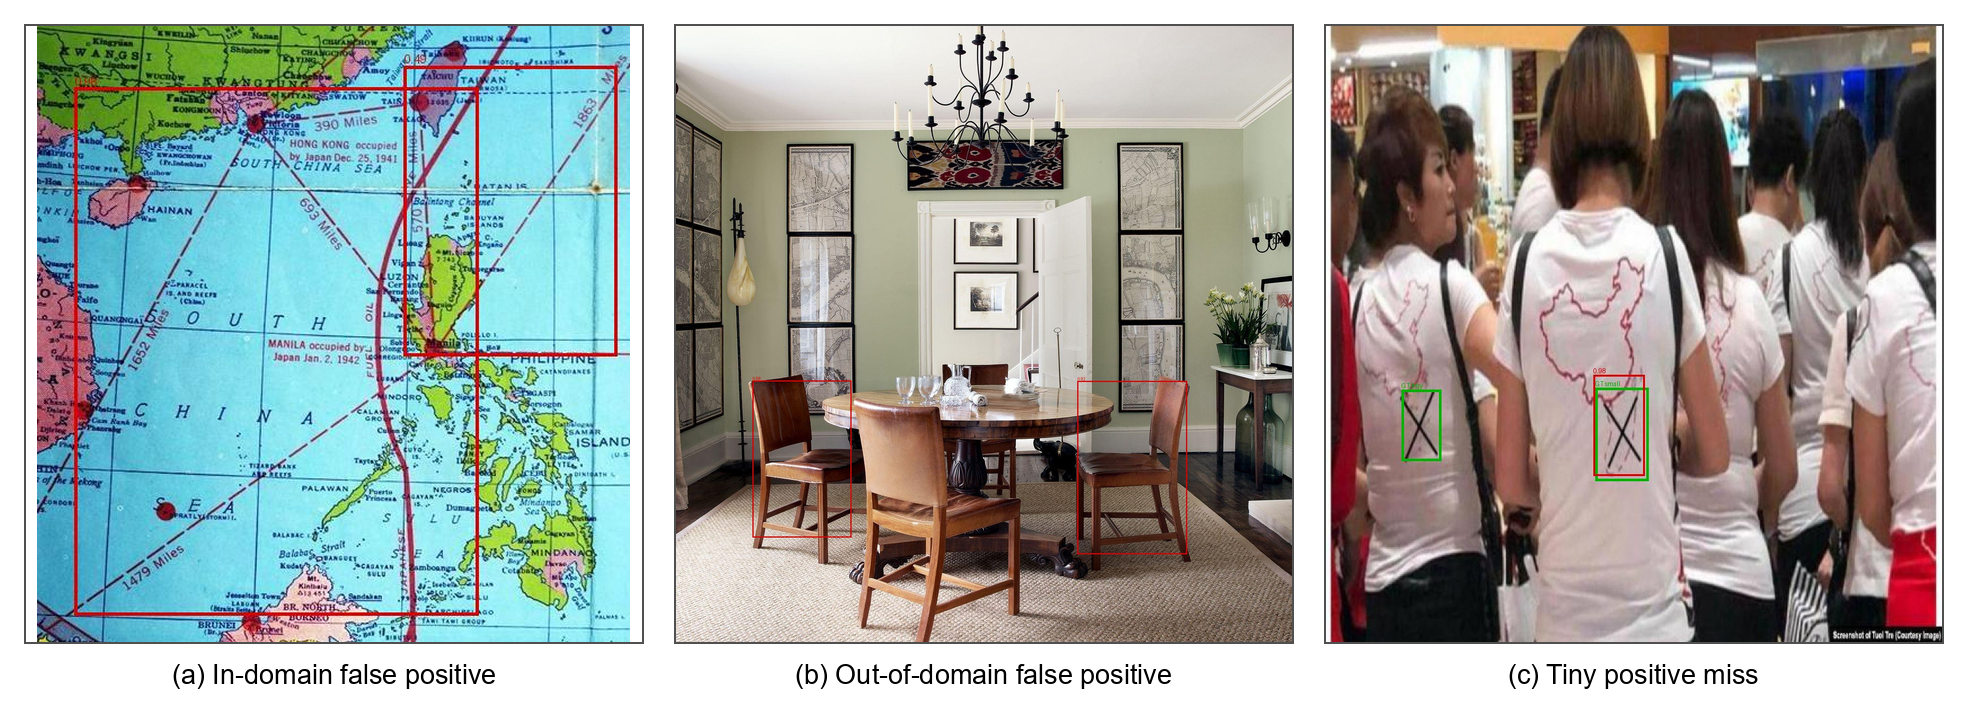
\includegraphics[width=\columnwidth]{fig3_error_examples.png}
\caption{Errors at $t=0.25$: (a) in-domain false positive, (b) out-of-domain false positive, and (c) tiny miss. Red and green boxes denote detections and ground truth.}
\label{fig:error_examples}
\end{figure}

Fig.~\ref{fig:error_examples} shows confusion with dashed map elements and unrelated structures, plus low-contrast or partial tiny targets. These cases suggest that remaining errors depend both on map semantics and on insufficient visual evidence at small scales.

\section{Discussion and Limitations}
In-domain negatives are essential: AP changes little while review-oriented false positives fall sharply. This gap shows that a positive-only test set can overstate operational usefulness. Model selection should therefore include group-specific FPR and FPPI, not AP alone, and deployment thresholds should be chosen for the available review budget. The two diagnostics answer different questions: FPR measures how many clean images are flagged, whereas FPPI measures how many candidate boxes a reviewer may inspect within them. YOLO models show competitive false-positive behavior, whereas Faster R-CNN provides the proposal interface needed to study HN-SARD. Metric priorities remain application dependent: low-review-load screening favors FPR@95TPR and FPPI, while localization favors AP75 and scale-specific AP.

For deployment, the reported $t=0.25$ is a diagnostic reference rather than a universal operating point. A system with scarce reviewer capacity should select its threshold from validation data and monitor in-domain negatives separately, since their errors dominate the remaining audit. The benchmark supports this process by retaining image scores and negative-group identities instead of collapsing all negative examples into one aggregate.

Tiny AP is diagnostic because validation and test contain few tiny objects, making small numerical differences unstable. Boxes support screening but do not measure individual-dash geometry. HN-SARD is evaluated only with Faster R-CNN R50-FPN, and the detector comparison is not exhaustive or a latency benchmark. Stronger proposal generation, higher-resolution training, and features better aligned with DINOv2 may improve the method. Future work should also test cross-source generalization, alternative image-score aggregation, and confidence intervals for tiny AP.

The HN-SARD results should therefore be interpreted as evidence for the region-distillation mechanism rather than a claim of universal superiority over one-stage detectors. The controlled comparison shows that a frozen foundation-model teacher can improve a proposal detector's localization and moderation behavior without inference-time teacher cost. Whether the same benefit transfers to dense prediction requires a different region-correspondence design and a separate controlled study.

Dataset coverage is another source of external-validity risk. Map styles, languages, compression pipelines, and publishing sources may shift after deployment, changing both positive appearance and the difficulty of in-domain negatives. Periodic evaluation on newly collected, source-disjoint data is consequently more informative than relying on a single fixed threshold indefinitely. Such evaluation should preserve the negative taxonomy so broad-domain robustness does not mask renewed map-specific confusion.

\section{Conclusion}
We present a public nine-dash-line benchmark and moderation-oriented protocol. Explicit negative data substantially reduces false positives, especially on map-like images, while HN-SARD improves AP and selected moderation metrics over Faster R-CNN. The benchmark and ablations provide a practical basis for cartographic-symbol moderation research.

\begin{thebibliography}{99}
\bibitem{ren2015faster}
S. Ren, K. He, R. Girshick, and J. Sun, ``Faster R-CNN: Towards real-time object detection with region proposal networks,'' in \emph{Proc. NeurIPS}, 2015.

\bibitem{lin2017fpn}
T.-Y. Lin, P. Dollar, R. Girshick, K. He, B. Hariharan, and S. Belongie, ``Feature pyramid networks for object detection,'' in \emph{Proc. CVPR}, 2017.

\bibitem{liu2016ssd}
W. Liu \emph{et al.}, ``SSD: Single shot multibox detector,'' in \emph{Proc. ECCV}, 2016.

\bibitem{redmon2016you}
J. Redmon, S. Divvala, R. Girshick, and A. Farhadi, ``You only look once: Unified, real-time object detection,'' in \emph{Proc. CVPR}, 2016.

\bibitem{wang2024yolov9}
C.-Y. Wang, I.-H. Yeh, and H.-Y. M. Liao, ``YOLOv9: Learning what you want to learn using programmable gradient information,'' arXiv:2402.13616, 2024.

\bibitem{wang2024yolov10}
A. Wang, H. Chen, L. Liu, K. Chen, Z. Lin, J. Han, and G. Ding, ``YOLOv10: Real-time end-to-end object detection,'' arXiv:2405.14458, 2024.

\bibitem{ultralytics2024yolo11}
Ultralytics, ``Ultralytics YOLO11,'' software documentation, 2024. [Online]. Available: \url{https://docs.ultralytics.com/models/yolo11/}

\bibitem{kisantal2019augmentation}
M. Kisantal, Z. Wojna, J. Murawski, J. Naruniec, and K. Cho, ``Augmentation for small object detection,'' arXiv:1902.07296, 2019.

\bibitem{shrivastava2016ohem}
A. Shrivastava, A. Gupta, and R. Girshick, ``Training region-based object detectors with online hard example mining,'' in \emph{Proc. CVPR}, 2016.

\bibitem{lin2017focal}
T.-Y. Lin, P. Goyal, R. Girshick, K. He, and P. Dollar, ``Focal loss for dense object detection,'' in \emph{Proc. ICCV}, 2017.

\bibitem{cheng2018dcr}
B. Cheng, Y. Wei, R. Feris, J. Xiong, W.-M. Hwu, T. Huang, and H. Shi, ``Decoupled classification refinement: Hard false positive suppression for object detection,'' arXiv:1810.04002, 2018.

\bibitem{hinton2015distilling}
G. Hinton, O. Vinyals, and J. Dean, ``Distilling the knowledge in a neural network,'' arXiv:1503.02531, 2015.

\bibitem{li2022rank}
G. Li, X. Li, Y. Wang, S. Zhang, Y. Wu, and D. Liang, ``Knowledge distillation for object detection via rank mimicking and prediction-guided feature imitation,'' in \emph{Proc. AAAI}, 2022.

\bibitem{caron2021dino}
M. Caron, H. Touvron, I. Misra, H. Jegou, J. Mairal, P. Bojanowski, and A. Joulin, ``Emerging properties in self-supervised vision transformers,'' in \emph{Proc. ICCV}, 2021.

\bibitem{oquab2023dinov2}
M. Oquab \emph{et al.}, ``DINOv2: Learning robust visual features without supervision,'' arXiv:2304.07193, 2023.

\bibitem{lin2014coco}
T.-Y. Lin \emph{et al.}, ``Microsoft COCO: Common objects in context,'' in \emph{Proc. ECCV}, 2014.
\end{thebibliography}

\end{document}
